\documentclass[10pt,a4paper]{article}
\usepackage[margin=0.78in]{geometry}
\usepackage{graphicx,booktabs,amsmath,hyperref,url}
\title{Learning-Augmented Page Replacement Under a Workload Shift}
\author{Student Name \quad Student ID}
\date{CSE-307 Operating Systems -- Section B}
\begin{document}
\maketitle

\begin{abstract}
This paper evaluates FIFO, LRU, Belady's optimal replacement, and a lightweight decision-tree eviction heuristic on three independently seeded synthetic traces. Each trace changes at its midpoint from locality-heavy references to broad random access. We report mean results and sample standard deviations, examining how working-set changes affect page faults and whether simple history features respond to the shift. Optimal provides an offline lower bound, not an implementable online policy.
\end{abstract}

\section{Problem framing}
Virtual memory allows a process to use a logical address space larger than physical memory, but a reference to a page not currently resident causes a page fault. When a frame is full, the replacement policy chooses a victim. FIFO is simple but ignores reuse, while LRU uses the recent past as a proxy for near-future reuse. Belady's optimal policy chooses the page whose next use is farthest away and is therefore useful as an offline comparison \cite{belady1966,mattson1970}. The course brief asks whether a lightweight learned layer can respond when the workload changes \cite{brief2026}.

\section{Implementation and learned component}
The Python program in `src/experiment.py` implements all four policies. The simulator records a hit vector and page-fault count for every reference. The learned policy uses a depth-4 decision tree, following the standard classifier interface described in the scikit-learn documentation \cite{sklearn2025}. For each resident candidate, its features are (i) age since last reference, (ii) frequency in the previous 64 references, and (iii) whether it was touched in the previous eight references. Training uses an independent seeded trace. Labels identify the candidate with the farthest next use in a 96-reference horizon. During evaluation, only current/history features are supplied.

This design is deliberately small and interpretable. It is also an important limitation: the labels use future information during training, so the result demonstrates a learned heuristic rather than a fully online production predictor.

\section{Experimental setup}
Three evaluation traces use seeds 307, 308, and 309. Each contains 1,000 references. References 0--499 are locality-heavy: 82\% of accesses select from a small hot set, with occasional sequential accesses. At reference 500, the distribution shifts to uniform random references over 32 pages. Each policy is tested with 4, 8, and 12 frames; the main comparison uses 8 frames. Each trace is replayed unchanged for every policy. The learned tree is trained once on an independent trace and held fixed. Per-seed traces and measurements are stored in `results/`.

\section{Results and analysis}
Table~\ref{tab:results} reports the mean and sample standard deviation of faults over three seeds. The generated figure shows the 8-frame mean fault counts for the two phases, with error bars of one sample standard deviation.

\begin{table}[h]
\centering
\caption{8-frame results from the seeded run.}
\label{tab:results}
\begin{tabular}{lrrrr}
\toprule
Policy & Local faults (mean $\pm$ SD) & Local hit ratio & Shifted faults (mean $\pm$ SD) & Shifted hit ratio\\
\midrule
FIFO & 138.3 $\pm$ 8.1 & 0.723 & 375.0 $\pm$ 9.6 & 0.250 \\
LRU & 110.0 $\pm$ 6.6 & 0.780 & 372.7 $\pm$ 16.2 & 0.255 \\
Optimal & 57.3 $\pm$ 1.5 & 0.885 & 231.7 $\pm$ 5.9 & 0.537 \\
Learned & 79.0 $\pm$ 2.6 & 0.842 & 383.7 $\pm$ 11.6 & 0.233 \\
\bottomrule
\end{tabular}
\end{table}

In the locality phase, LRU benefits from repeated hot-page references because recent use predicts reuse. Optimal has the fewest faults because it sees the future and serves as a lower bound. After the shift, the larger effective working set drives a substantial increase in faults for every policy. The learned heuristic has the lowest locality-phase mean faults among the implementable policies in this setup, but its shifted-phase hit ratio is below FIFO and LRU. Its fixed model does not generalize equally well to the new distribution, illustrating the risk of distribution mismatch.

\begin{figure}[h]
\centering
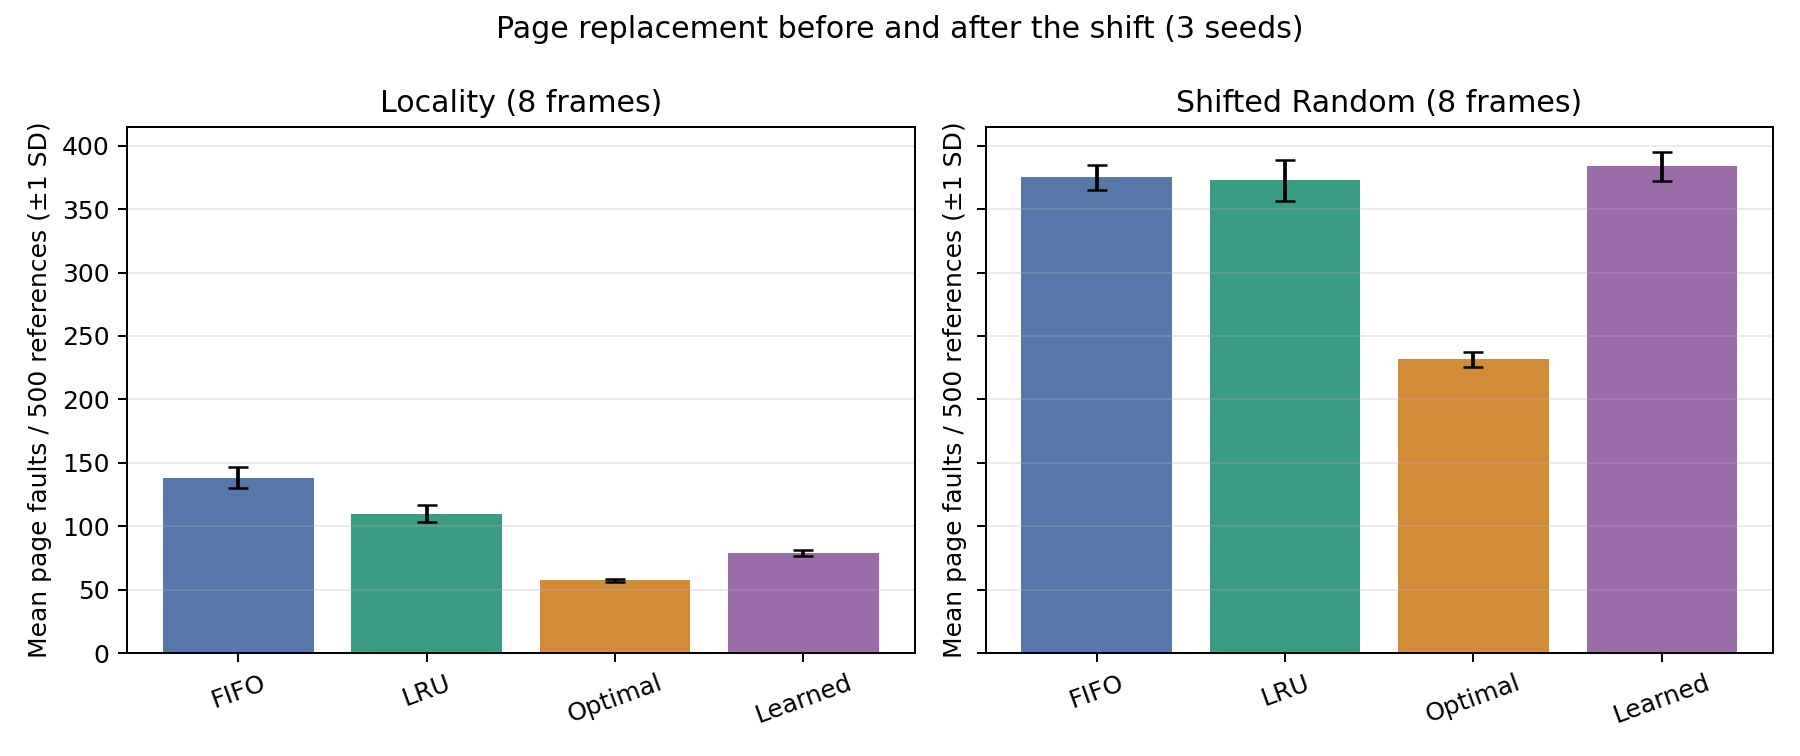
\includegraphics[width=0.9\linewidth]{../results/page_faults.png}
\caption{Fault counts before and after the distribution shift for eight frames.}
\end{figure}

\section{Conclusion}
Across three generated seeds, the broad random phase consistently produces substantially more faults than the locality phase. The learned policy performs best among the online policies in the locality phase but loses that advantage after the shift. These synthetic results illustrate how a fixed learned rule can be sensitive to changing distributions. More seeds, online training labels, and real traces would be needed before making deployment claims.

\bibliographystyle{plain}
\bibliography{references}
\end{document}
